% !TeX program = lualatex

% Author: Malte, DE7LMS
% Year: 2021
% ???
\documentclass[convert = false, border=5pt]{standalone}
\input{../common/settings.tex}

\begin{document}
% \begin{tikzpicture}[
%     line join=round
%   ]

%   \draw[very thick]
%     (0,0) -- (2,0) -- (1,{sqrt(3)}) -- cycle;
% \end{tikzpicture}

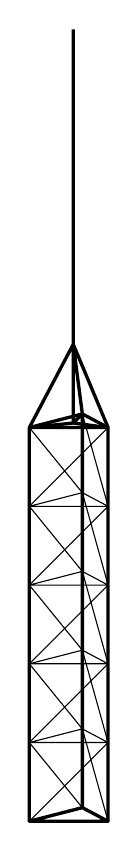
\begin{tikzpicture}[
    x={(1cm,0cm)},
    y={(.2cm,.2cm)},
    z={(0cm,1cm)},
    line join=round
  ]

  \draw[very thick]
    (0,0,5) -- (0,0,10)
    (1,0,5) -- (1,0,10)
    (1/2,{sqrt(3)/2},5) -- (1/2,{sqrt(3)/2},10)
    %
    (0,0,10) -- (1/2,{sqrt(3)/6},10)
    (1,0,10) -- (1/2,{sqrt(3)/6},10)
    (1/2,{sqrt(3)/2},10) -- (1/2,{sqrt(3)/6},10)
    %
    (0,0,10) -- (1/2,{sqrt(3)/6},11)
    (1,0,10) -- (1/2,{sqrt(3)/6},11)
    (1/2,{sqrt(3)/2},10) -- (1/2,{sqrt(3)/6},11)
    %
    (1/2,{sqrt(3)/6},10) -- (1/2,{sqrt(3)/6},15)
    ;
  \foreach \z in {6,7,...,9}
    \draw
      (0,0,\z) -- (1,0,\z) -- (1/2,{sqrt(3)/2},\z) -- cycle;
  \foreach \z in {5,10}
    \draw[very thick]
      (0,0,\z) -- (1,0,\z) -- (1/2,{sqrt(3)/2},\z) -- cycle;
  \foreach \z in {5,6,...,9}
    \draw
      (0,0,\z) -- (1,0,\z+1)
      % (1,0,\z) -- (0,0,\z+1)
      %
      (1,0,\z) -- (1/2,{sqrt(3)/2},\z+1)
      % (1/2,{sqrt(3)/2},\z) -- (1,0,\z+1)
      %
      (1/2,{sqrt(3)/2},\z) -- (0,0,\z+1)
      % (0,0,\z) -- (1/2,{sqrt(3)/2},\z+1)
      ;
\end{tikzpicture}

\end{document}